%!TEX root =  main.tex
\newcommand{\one}[1]{\mathbb{I}_{\{#1\}}}
\newcommand{\Pside}{\P_{\mathrm{side}}\xspace}
\newcommand{\PSAP}{\P_{\mathrm{SAP}}\xspace}
\renewcommand{\P}{\mathcal{P}}

In this section we establish that SAP with weak dominance property is `regret equivalent' to an instance of MAB with side-information and the corresponding algorithm for MAB can be suitably imported to solve SAP efficiently.   

\if0
\todoc[inline]{I am thinking that maybe we should skip this general section
and just do the specific reduction as shown below.}
We start with the concept of regret equivalence, which we define for classes of partial monitoring problems.
First, we need some extra notation: Recall that at the end of \cref{sec:background} we agreed that 
a partial monitoring problem can be specified as a 3-tuple $(\A,\Y,\Theta)$ where the elements of $\Theta$ are pairs $(p,r)$,
where for each $a\in \A$ action, $p(\cdot;a)$ is a probability distribution over $\Y$ and $r: \A \to \R$.
Now, let $\Pi(\P)$ denote the set of policies for some partial monitoring problem $\P = (\A,\Y,\Theta)$,
let $\Regret_T(\pi,\theta)$ denote the expected regret of policy $\pi$ on problem instance $\theta\in \Theta$,
and let $\Regret_T^*(\P) = \inf_{\pi\in \Pi(\P)}\sup_{\theta\in \Theta} \Regret_T(\pi,\theta)$ denote the minimax regret on $\P$.

Now let $\P_1 = (\A_1,\Y_1,\Theta_1)$, $\P_1 = (\A_2,\Y_2,\Theta_2)$ be partial monitoring problems.
We say that \emph{$P_1$ is $P_2$-hard}, 
denoted by $P_1 \succeq P_2$, if for any $\pi_1\in \Pi(\P_1)$ policy of $\P_1$ there exists a policy $\pi_2\in \Pi(\P_2)$ of $\P_2$
such that for any $\theta_2\in \Theta_2$ there exists an instance $\theta_1\in \Theta_1$ such that $\Regret_T(\pi_1,\theta_1)\ge \Regret_T(\pi_2,\theta_2)$. An immediate corollary of the definition, justifying the definition, is the following:
\begin{proposition}
If $\P_1\succeq \P_2$ then $\Regret_T^*(\P_1)\ge \Regret_T^*(\Pi_2)$.
\end{proposition}
\begin{proof}
Fix some $\epsilon>0$ and 
let $\pi_1^*\in \Pi(\P_1)$ be an $\epsilon$-minimax-optimal policy of $\P_1$: 
$\sup_{\theta_1\in\Theta_1} \Regret_T(\pi_1^*,\theta_1) \le \Regret_T^*(\P_1)+\epsilon$.
Let $\pi_2^*$ be the policy whose existence follows by the assumption $\P_1\succeq \P_2$.
Let $\theta_2^*\in \Theta_2$ be an instance in $\P_2$ such that 
$\Regret_T(\pi_2^*,\theta_2^*)\ge \sup_{\theta_2\in \Theta_2} \Regret_T(\pi_2^*,\theta_2)-\epsilon$
and let $\theta_1^*\in \Theta_1$ in $\P_1$ whose existence is implied by $\P_1\succeq \P_2$.
Then,
\begin{align*}
 \Regret_T^*(\P_2) &= 
\inf_{\pi_2\in \Pi(\P_2)} \sup_{\theta_2\in \Theta_2} \Regret_T(\pi_2,\theta_2)
\le \sup_{\theta_2\in \Theta_2} \Regret_T(\pi_2^*,\theta_2) 
\le  \Regret_T(\pi_2^*,\theta_2^*)+\epsilon \\
& \le  \Regret_T(\pi_1^*,\theta_1^*)+\epsilon
\le \sup_{\theta_1\in \Theta_1} \Regret_T(\pi_1^*,\theta_1)+\epsilon
\le \Regret_T^*(\P_1) +2\epsilon\,.
\end{align*}
Letting $\epsilon\to 0$ finishes the proof.
\end{proof}
We call two problems \emph{$\P_1,\P_2$ regret-equivalent} if $\P_1$ is $\P_2$-hard and also $\P_2$ is $\P_1$-hard.
It follows immediately that if $\P_1,\P_2$ are regret equivalent then they have the same minimax regret.

A simple way of guaranteeing that a problem $\P_1$ is $\P_2$-hard if we can transform problem instances of $\P_2$ into 
problem instances of $\P_1$ while keeping the reward differences between the action-rewards the same (i.e., allowing the reward to be shifted by a constant).
Formally, we have the following proposition:
\begin{proposition}
Let $\P_i = (\A_i,\Y_i,\Theta_i)$, $i=1,2$ be partial monitoring problems.
Then, $\P_1\succeq \P_2$ holds if there exists $f_{\A}:\A_2\to \A_1$, $f_{\Y}: \Y_2 \to \Y_1$ bijections and $f_{\Theta}:\Theta_2\to \Theta_1$ such that if $(p,r) = f_{\Theta}(p',r')$ for some $(p',r')\in \Theta_2$ then
for any $a',a''\in \A_2$, $y'\in \Y$,
$p'(y';a') = p(f_\Y(y'),f_\A(a'))$ and $r'(a')-r'(a'') = r(f_\A(a')) - r(f_\A(a''))$.
\end{proposition}
\begin{proof}
The proof follows directly from two simple observations 
that hold for any instance $\theta_2 = (p',r')$ of $\P_2$: 
First, if $a_2^*$ is an optimal action for $\theta_2$
then $a_1^*=f_\A(a_2^*)$ is an optimal action for instance $(p,r) = f_\Theta(\theta_2)$.
Second, any policy $\pi_1$ of $\P_1$ can be translated using the maps $f_\A$ and $f_\Y$ into a policy $\pi_2$ of $\P_2$ (regardless of $\theta_2$) such that
for any $t\ge 1$,
$P_{\pi_2,\theta_2,t}$ is the push-forward distribution 
of $P_{\pi_1,\theta_1}$ under $f_t:(\A_2\times \Y_2)^t \to (\A_1\times \Y_1)^t$
defined by $f_t(a_1',y_1',\dots,a_t',y_t') = (f_\A(a_1'),f_\Y(y_1'),\dots,f_\A(a_t'),f_\Y(y_t'))$. 
Here $\pi_2(a'_t|a_1',y_1',\dots,a_t',y_t') = \pi_1( f_\A(a_t')| f_\A(a_1'),f_\Y(y_1'),\dots,f_\A(a_t'),f_\Y(y_t'))$ and recall that $P$ is called the push-forward measure of $Q$ under $f:\mathrm{dom}(Q)\to \mathrm{dom}(P)$ if $P$ is the distribution of $f(X)$ where $X\sim Q$.
Both claims can be seen to hold by a simple direct calculation whose details are left 
to the reader.
From the two claims it follows that $\Regret_T(\pi_1,\theta_1)
= \Regret_T(\pi_2,\theta_2)$, showing that $\P_1$ and $\P_2$ are indeed
regret equivalent.
\end{proof}

\todo[inline]{Here is the actual reduction. Maybe let's just keep this part?}
\fi



\begin{wrapfigure}{r}{6cm}
	\centering
	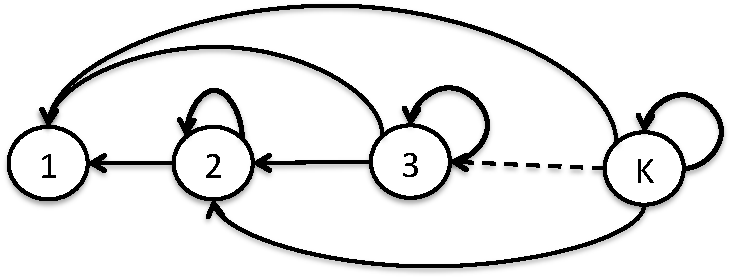
\includegraphics[scale=.4]{../Figures/SideInfoGraph.pdf}
	\caption{Side observation graph $G_S$. \todoc[inline]{Keeping the fig just in case.}}
	\label{fig:SideObservationGraph]}
\end{wrapfigure} 

%Let us now show how to reduce SAP under strong dominance to a specific 
%bandit with side-observations.
Let $\PSAP$ be the set of SAPs with action set $\A = [K]$.
The corresponding bandit problems will have the same action set,
while for action $k\in [K]$ the neighborhood set is $\mathcal{N}(k) = [k]$.
Take any instance $(P,c)\in \PSAP$ and let $(Y,Y^1,\dots,Y^K) \sim P$ be the 
unobserved state of environment in round $s$.
We let the reward distribution for arm $k$ in the corresponding bandit problem
be a shifted Bernoulli distribution.
In particular, the cost of arm $k$ follows the distribution of 
$\one{Y^k\ne Y^1} + C_k$ (we use costs here to avoid flipping signs).
The costs for different arms are defined to be independent of each other.
Let $\Pside$ denote the set of resulting bandit problems and let $f:\PSAP \to \Pside$
be the map that transforms SAP instances to bandit instances by following the
transformation that was just described.
\todoc[inline]{
Ok, so if they are independent of each other, then the joint distributions will not be 
same as if they were not independent of each other.
Independence may lose information (e.g., may increase variance?).
If we define them not to be independent of each other, we will need to be careful
with the algorithms defined for bandits with side-observation: Do they use
(in their proof) independence of rewards underlying different arms?
I would think that they are not.
The downside of not defining independent rewards is that the specification of
bandits with side observations must allow this -- complicating things a bit in the background.
Another executive decision we should make is whether we like to see both costs and 
rewards.
}

Now let $\pi\in \Pi(\Pside)$ be a policy for $\Pside$.
Policy $\pi$ can also be used on any $(P,c)$ instance in $\PSAP$ in an obvious way:
In particular, given the history of actions and states $A_1,U_1,\dots,A_t,U_t$
in $\theta=(P,c)$ where $U_s = (Y_s,Y_s^1,\dots,Y_s^{K})$ such that 
the distribution of $U_s$ given that $A_s=a$ is $P$ marginalized to $\Y^{a}$,
the next action to be taken is 
$A_{t+1}\sim \pi(\cdot| A_1, V_1,\dots,A_t,V_t)$, where
$V_s = (\one{Y_s^1\ne Y_s^1}+C_1,\dots,\one{Y_s^1\ne Y_s^{A_s}}+C_{A_s})$. Let the resulting policy be denoted by $\pi'$.
The following can be checked by simple direct calculation:
\begin{proposition}
If $\theta \in \TWD$, then the regret of $\pi'$ on $f(\theta)\in \Pside$
is the same as the regret of $\pi$ on $\theta$. \todoc[inline]{We should probably add this
calculation?}
\end{proposition}
This implies that $\Regret_T^*(\TWD)\le \Regret_T^*(f(\TWD))$.

Now note that this reasoning can also be repeated in the other ``direction'': 
For this, first note that the map $f$ has a right inverse $g$ 
(thus, $f\circ g$ is the identity over $\Pside$)
and if $\pi'$ is a policy for $\PSAP$, 
then $\pi'$ can be ``used''  on any instance $\theta\in \Pside$
via the ``inverse'' of the above policy-transformation:
Given the sequence $(A_1,V_1,\dots,A_t,V_t)$ where 
$V_s= (B_s^1+C_1,\dots,B_ s^{K}+C_s)$ is the vector of costs for round $s$
with $B_s^k$ being a Bernoulli with parameter $\gamma_k$,
let $A_{t+1} \sim \pi'( \cdot| A_1,W_1,\dots,A_t,W_t)$ where
$W_s = (B_s^1,\dots,B_s^{A_s})$. Let the resulting policy be denoted by $\pi$.
Then the following holds:
\begin{proposition}
Let $\theta \in f(\TWD)$. Then the regret of policy $\pi$ on $\theta\in f(\TWD)$ is the same
as the regret of policy $\pi'$ on instance $f^{-1}(\theta)$.
\end{proposition}
Hence, $\Regret_T^*(f(\TWD))\le \Regret_T^*(\TWD)$.
In summary, we get the following result:
\begin{corollary}
$\Regret_T^*(\TWD) = \Regret_T^*(f(\TWD))$. 
\end{corollary}
\todoc[inline]{So this could in theory be used for upper and lower bounds.. 
However, $\Pside$ is really special (because of the fixed costs) -- hence it is unclear 
whether existing lower bounds, for example, would apply.
The next step could be to describe policies for bandits
with side observation starting from our paper with Yifan.
We have two types of policies.
One is asymptotically optimal, the other is minimax optimal.
Can we have a single policy in our special problem that would be simultanously 
optimal in both cases? What happens when only weak dominance
is satisfied?}

\if0
At the price of abusing notation 
we simplify the notation by dropping the indices from $f_{\A}, f_{\Y}$ and $f_{\Theta}$ (the identity of the appropriate map can be inferred from its argument).
Pick any policy $\pi_1\in \Pi_1$.s
First we define the policy corresponding to $\pi_1$.
Recall that a policy maps histories to distributions over actions.
Taking a history $(a_1,y_1,\dots,a_t,y_t)\in (\A_2\times \Y_2)^t$ ($t\ge 0$),
for $a_{t+1}\in \A_2$ we define the probability of taking $a_{t+1}$ by $\pi_2$, in notation,
 $\pi_2(a_{t+1}|a_1,y_1,\dots,a_t,y_t)$, as
 $\pi_2(a_{t+1}|a_1,y_1,\dots,a_t,y_t) = \pi_1(f(a_{t+1})|f(a_1),f(y_1),\dots,f(a_t),f(y_t))$.
Pick any instance $\theta_2 = (p',r')\in \Theta_2$ and let $(p,r) = \theta_1  = f( \theta_2)$.
The probability distribution over histories $\Y_1 \times \A_1$ generated by $\pi_1$ and $\theta_1$
\fi



